%%%% Proceedings format for most of ACM conferences (with the exceptions listed below) and all ICPS volumes.
\documentclass[sigconf]{acmart}
\usepackage{graphicx, wrapfig}
\graphicspath{{imgs/}}
\usepackage{lipsum}
\usepackage{stfloats}
\usepackage{enumerate}
\usepackage[most]{tcolorbox}
\usepackage[english,ngerman,brazilian]{babel}

\newtcolorbox[blend into=figures]{card}[2][]{enhanced,
  float=tbp,title={#2},
  colframe=gray!75!black,olback=yellow!5!white,#1
}


\settopmatter{printacmref=false}
\setcopyright{none}
\renewcommand\footnotetextcopyrightpermission[1]{}
\pagestyle{plain}
\captionsetup{justification   = raggedright,
              singlelinecheck = false}
\newcommand{\source}[2]{\raggedleft{}\vspace*{-7mm}\caption*{ \textmd{\scriptsize{Dados: {#1}.\hfill Ferramenta:{#2}}}}}
\def\BibTeX{{\rm B\kern-.05em{\sc i\kern-.025em b}\kern-.08emT\kern-.1667em\lower.7ex\hbox{E}\kern-.125emX}}

% end of the preamble, start of the body of the document source.
\begin{document}

%
% The "title" command has an optional parameter, allowing the author to define a "short title" to be used in page headers.
\title[Fronteiras da Transferência de Aprendizado: uma revisão sistemática com enfoque meta-analítico]{Fronteiras da Transferência de Aprendizado: \\
uma revisão sistemática com enfoque meta-analítico}
%

\author{Fred Guth}
\email{fredguth@fredguth.com}
\affiliation{%
  \institution{Departamento de Ciência de Computação, Universidade de Brasília}
  \postcode{70.910-900}
  \city{Brasília}
  \state{DF}
  \country{Brazil}
}

\renewcommand{\shortauthors}{Guth, F.}

\begin{abstract}
  Humanos e animais conseguem aprender com poucas amostras \cite{goodfellow} e apresentam extraordinária capacidade de generalização que os algoritmos de aprendizagem de máquina ainda estão longe de alcançar. Os modelos mais bem sucedidos da atualidade exigem uma enormidade de dados bem rotulados que são caros e difíceis de obter, tornando-se hoje um dos maiores empecilhos para aplicações práticas. Tais fatos apontam para o grande potencial da área de Transferência de Aprendizado, que tem por objetivo aproveitar o conhecimento obtido em uma atividade para aprender mais eficientemente outras, que guardem alguma relação com a primeira. O presente estudo visa apresentar uma revisão sistemática da literatura e identificar, com embasamento quantitativo, as principais contribuições para a área. Além disso, usamos medidas de acoplamento bibliográfico para identificar trabalhos na fronteira do conhecimento e fizemos uma análise textual, em resumos e palavras-chave, comparando estes com os "clássicos" da área de forma a mapear para que direção a pesquisa avança.  
\end{abstract}


\begin{CCSXML}
<ccs2012>
 <concept>
 <concept_id>10010147.10010257.10010258.10010262.10010277</concept_id>
 <concept_desc>Computing methodologies~Transfer learning</concept_desc>
 <concept_significance>500</concept_significance>
 </concept>
</ccs2012>
\end{CCSXML}
\ccsdesc[500]{Computing methodologies~Transfer learning}

\keywords{transferência de aprendizado, revisão sistemática, enfoque meta-analítico}


\maketitle


\section{Introdução} 
  Recentes avanços em Aprendizagem de Máquina tornam possíveis aplicações que são capazes de reconhecer pessoas, lugares e objetos com acurácia super-humana\cite{fei}, diagnosticar câncer de pele tão bem quanto dermatologistas\cite{skin_cancer},  ver através de paredes usando sinais de rádio\cite{wifi}, entre tantas outras. Apesar de tanto sucesso, os modelos mais bem sucedidos da atualidade exigem uma enormidade de dados bem rotulados que são caros e difíceis de obter, pois, em geral, o jeito padrão de se treinar modelos é sempre começar \emph{tabula rasa}, ou seja, com uma inicialização aleatória dos parâmetros. 
  
  Aprender assim, a partir do nada, é contrário à forma como os humanos o fazem. Em nosso dia a dia, transferimos conhecimento a todo momento. Saber tocar piano, facilita aprender tocar órgão. Reconhecer maçãs talvez ajude a reconhecer peras. Pessoas conseguem inteligentemente aplicar conhecimento prévio para resolver novos problemas com maior eficácia e eficiência\cite{PanYang}. Algoritmos de aprendizagem de máquina ainda estão longe de alcançar essa extraordinária capacidade de generalização\cite{goodfellow}. Estudos recentes~\cite{DBLP:journals/corr/JiaL17}, mostram que os algoritmos atuais não generalizam bem além de dados vistos durante o treinamento.
  \begin{figure}[h]
    \includegraphics[width=\columnwidth]{citacoes_por_ano2.pdf}
    \source{Web of Science (março/2019)}{Excel}
    \caption{Evolução dos número de citações de artigos em Tranferência de Aprendizagem nos últimos 10 anos.}
    \label{fig:citacoes_por_ano}
  \end{figure}
  
  Tais fatos apontam  o grande potencial ainda inalcançado da área de Transferência de Aprendizado (TL\footnote{Do inglês \emph{Transfer Learning}}), que tem por objetivo aproveitar o conhecimento obtido em uma atividade para aprender mais eficientemente outras, que guardem alguma relação com a primeira.
  
  Na prática, entretanto, TL ainda é tratada de uma forma \textit{ad hoc}, sendo os métodos de transferências meras extensões dos algoritmos de aprendizado utilizados \cite{torrey}.Essa dicotomia entre a importância do problema e a inexistência de práticas e teorias consolidadas, tornam TL um campo promissor e interessante para pesquisa. 
  
  Essa é a opinião de especialistas renomados, como Andrew Ng:
  \begin{quote} "Transferência de Aprendizado será o próximo motor do sucesso comercial com Aprendizado de Máquinas." \hfill ---Andrew Ng, Tutorial NIPS 2016 \cite{ANg}
  \end{quote}

  Portanto, não é de se estranhar o crescente interesse pelo assunto (vide \S\ref{sec:panorama} e figura \ref{fig:citacoes_por_ano}).  

  \subsection{Objetivo}
   Esta pesquisa quer responder duas perguntas:
    \begin{enumerate}
      \item{Quais são as fronteiras do conhecimento em Transferência de Aprendizagem?}
      \item {É possível embasar essa avaliação em dados bibliométricos?}
    \end{enumerate}
    Para responder estas perguntas é preciso, antes, analisar a literatura do tema, revelar as principais contribuições e como se relacionam.
  
  \subsection{Contribuições}
    Para chegar a fronteira é preciso antes integrar a literatura do tema e revelar as principais contribuições e como se relacionam.
    \lipsum[3]
  
  \subsection{Visão Geral e Organização do Artigo}
  \lipsum[3]
  \subsection{Trabalhos Relacionados}
  \lipsum[2]
\section{Método: Revisão com Enfoque Meta-Analítico Consolidado}
Na presente pequisa utilizamos o método de revisão sistemática da Teoria do Enfoque Meta-Analítico (TEMAC) ~\cite{Mariano}, que visa oferecer um embasamento quantitativo para a escolha da literatura. Apesar do nome, TEMAC não deve ser confundida com Meta-Análise, pois o foco desta é gerar conhecimento por meio de dados empíricos secundários, enquanto o daquela é oferecer uma sistematização da escolha bibliográfica.

A abordagem TEMAC é dividida em 3 etapas: 
\begin{enumerate}[a)]
  \item preparação da pesquisa;
  \item apresentação e inter-relação dos dados;
  \item detalhamento, modelo integrador e validação por evidências.
\end{enumerate}

\subsection{Preparação da Pesquisa}
\begin{figure}[htp]
\begin{tcolorbox}[colback=yellow!5!white,colframe=gray!75!black,title={Results: 1,279 (from Web of Science Core Collection)}]
  \begin{verbatim}
  You searched for: 
  TOPIC: ("transfer learning")
  Refined by: 
  WEB OF SCIENCE CATEGORIES: 
    ( COMPUTER SCIENCE ARTIFICIAL INTELLIGENCE )
  AND LANGUAGES: ( ENGLISH ) 
  AND RESEARCH AREAS: ( COMPUTER SCIENCE )
  Timespan: 2009-2019. 
  Indexes: SCI-EXPANDED, CPCI-S.
  \end{verbatim}

\end{tcolorbox}
\caption{Parâmetros de busca na base \emph{Web of Science}.}
\end{figure}


etapa 1.
WoS busca
etapa 2.
2.a análise das revistas mais relevantes
2.b análise das revistas que mais publicam
2.c evolução do tema ano a ano
2.d documentos mais cidados
2.e autores mais publicaram vs mais citados
2.f países que mais publicaram
2.g conferências que mais contribuíram
2.h organizações mais publicaram
2.i agências que mais financiam
2.j áreas que mais publicam
2.l frequencia das palavras chave

etapa 3. 
novos índices bibliométricos que detectam colégios invisíveis 

(co-citação, acoplamento).

  \begin{itemize}
    \item{\textbf{Análise de Co-citações}: co-citation analysis is advantageous for mapping the intellectual heritage of a particular field on the basis of high-impact publications, but tends to neglect the publication dynamics at the forefront of research. Bibliographic coupling, in contrast, cap- tures more recent contributions, including the classics of tomorrow, so to speak, however, this method has a blind spot with regard to the history of an intellectual field.
    \begin{figure}[h]
      \fbox{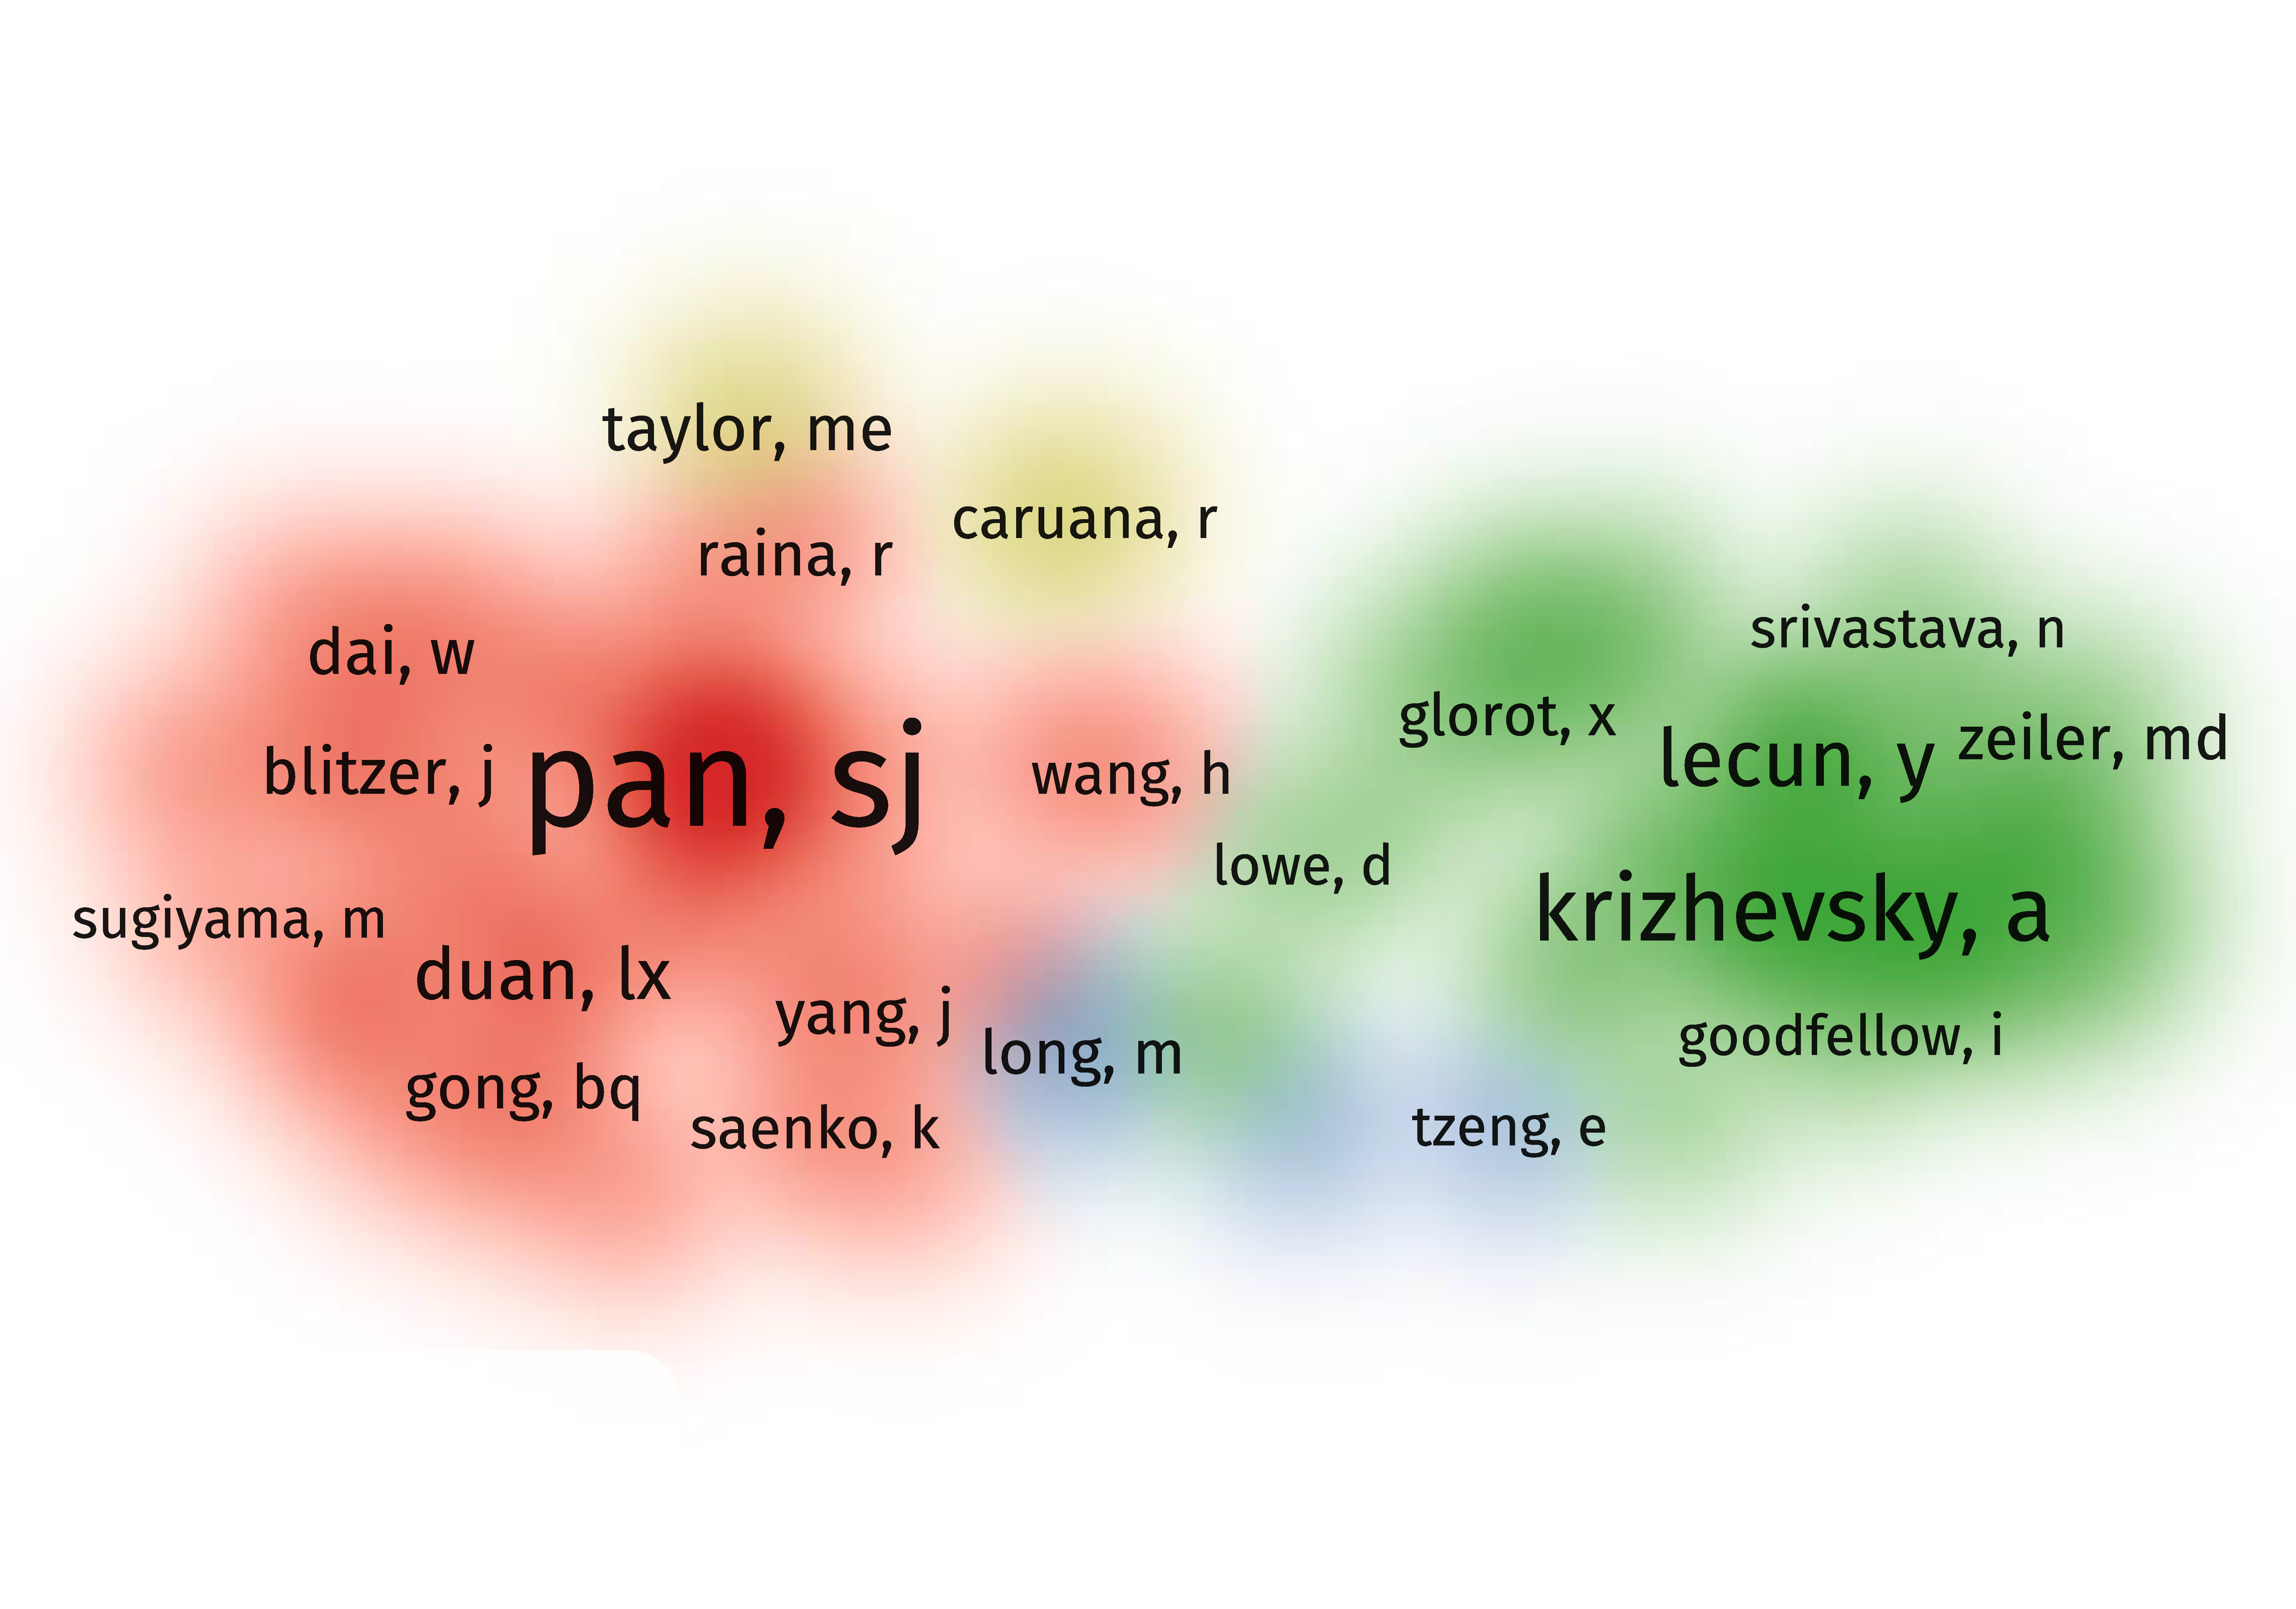
\includegraphics[width=\columnwidth]{completo-4clusters}}
      \source{Web of Science (março/2019)}{VosViewer\protect{~\cite{VOSviewer}}}
      \caption{Núcleos de conhecimento obtidos pela análise de co-citações. Os diferentes grupos representam autores que normalmente são co-citados nos 1268 artigos resultantes da busca realizada.}
      \label{fig:classicos}
    \end{figure}
    A co-citation is defined as the frequency with which two docu- ments1 are cited together in the literature (Small 1973). Documents are thus co-cited if they are included in the same reference list.}
    \item{\textbf{Análise de Acoplamento Bibliográfico}: bibliographic coupling is said to occur when two documents have at least one reference in common (Kessler 1963). Documents are thus coupled if their bibliographies overlap.}
    \item{\textbf{Análise Textual}}
  \end{itemize}
  co-citation is a similarity relationship between two cited publications, bibliographic coupling is a measure of association between two citing publica- tions 

 co-citation analysis lends itself to tracing the intellectual roots of an academic field through the identification of its foundational works. The older a document, the longer the period in which it can have accumulated citations. Compared with the ‘classics’ of an aca- demic field, more recent publications have had less time to leave their marks, regardless of their potential to become classic works in the future. In view of that, most researchers who employ co-citation analysis acknowledge that the method is biased towards ‘the past’ .
  
  In con- trast, bibliographic coupling is suitable for detecting current trends and future priorities as they are reflected at the forefront of research.
  % \subsection{Sumarização}
\section{Revisão da Literatura}
  \subsection{Transferência de Aprendizagem}
  \lipsum[3]
  \subsection{Um breve histórico}
  Pesquisa em transferêcia de conhecimento tem atraído mais e mais atenção desde 1995, quando foi tema de  um workshop na NIPS-95 que discutiu a necessidade de métodos de aprendizado de máquina que retém e reusam conhecimento previamente obtido\cite{sinno}. 
  \lipsum[2]
  \subsection{O panorama da produção científica na área}\label{sec:panorama}
  \lipsum[1]
  
  

 
  \subsection{Os Clássicos}
  % \begin{figure*}[b]
  %   \centering
  %   \fbox{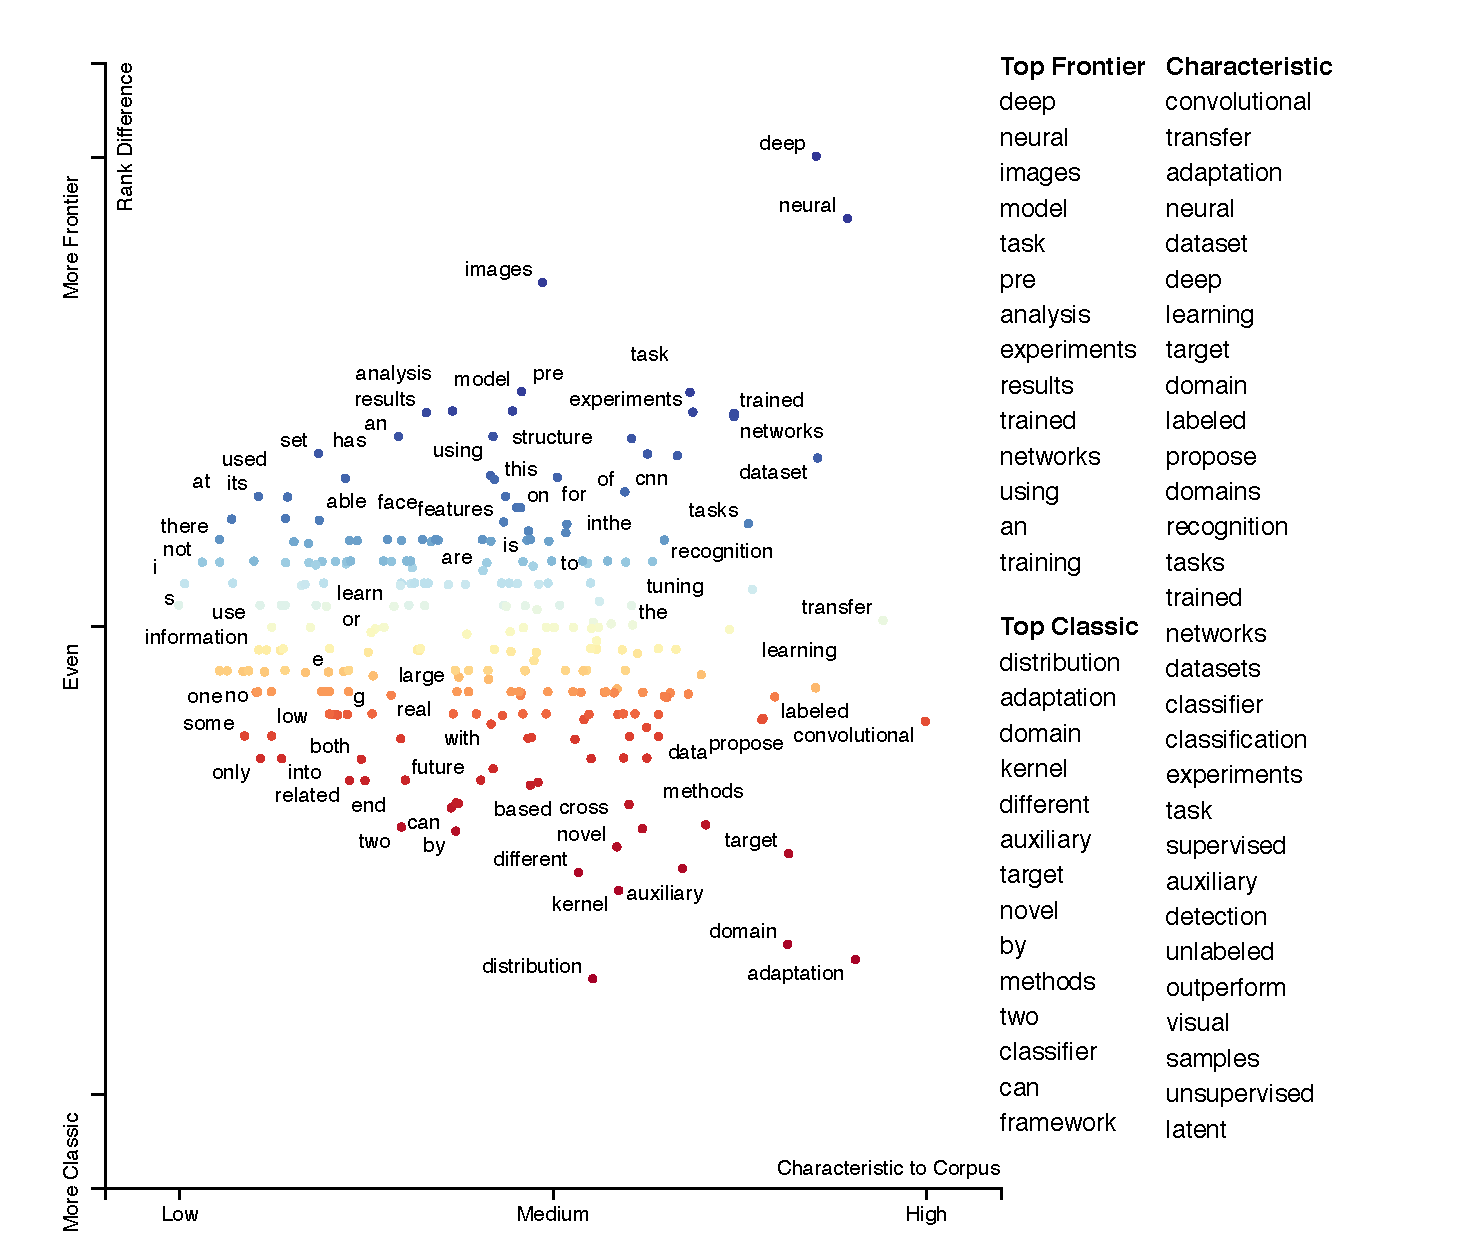
\includegraphics[width=\dimexpr \textwidth-2\fboxsep-2\fboxrule\relax, height= 12cm]{Frontier.pdf}}
  %   \caption{} \label{fig:studysite}
  % \end{figure*}

  \lipsum[3]
  \begin{figure}
    \fbox{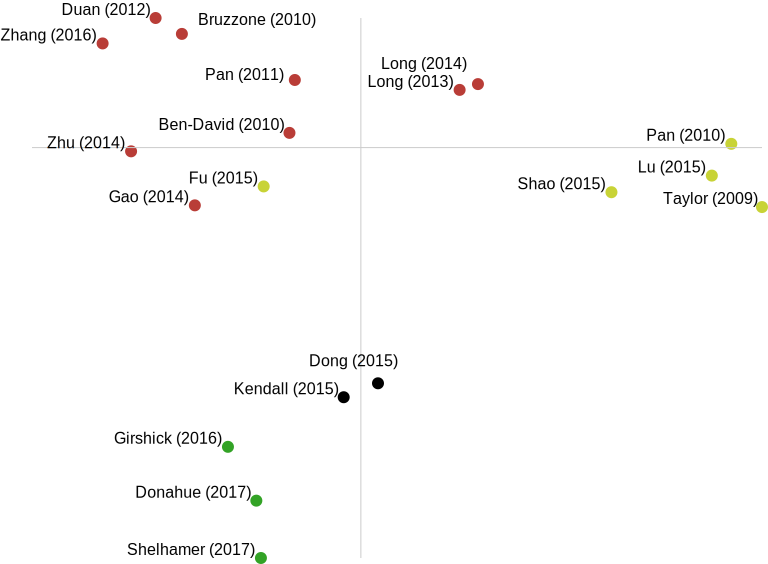
\includegraphics[width=\columnwidth]{top20_scatter.pdf}}
    \caption{} \label{fig:studysite}
  \end{figure}
  
  \subsection{A Fronteira}
  \lipsum[2]
  \begin{figure}
    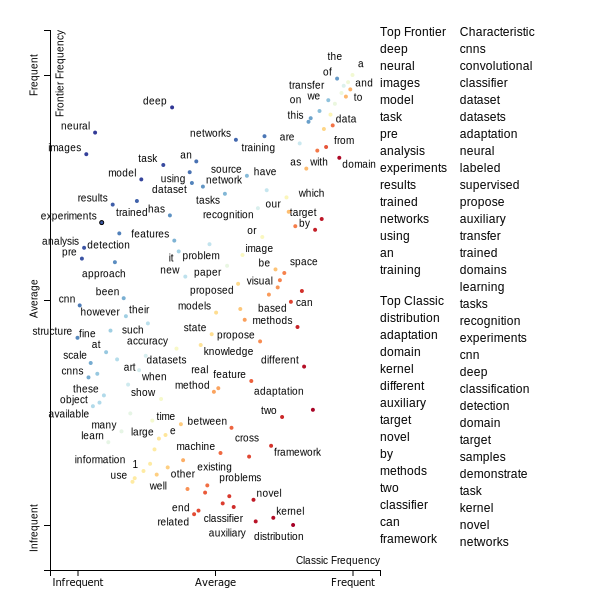
\includegraphics[width=\columnwidth]{frontier3.pdf}
    \caption{} \label{fig:studysite}
  \end{figure}

\section{Problemas em Aberto}
\lipsum[3]
\section{Conclusão}
\lipsum[3]
\bibliographystyle{ACM-Reference-Format}
\bibliography{references}
\end{document}
